As mentioned in the previous section we need a function to determine if changed made to the preconditioner was an improvement. Because this part of the algorithm is especially important, we will test three different improvement functions, for four different seeds each. The improvement functions will described in the following subsections.

\subsubsection{MEAN improvement function}
The first improvement function is the MEAN improvement function. It will accept a change made to the preconditioner if the mean solver iteration count of the preconditioned systems is lower than the previous mean solver iteration count.
\subsubsection{MEDIAN improvement function}
The second improvement function is the MEDIAN improvement function. It will accept a change made to the preconditioner if the median solver iteration count of the preconditioned systems is lower than the previous median solver iteration count.
\subsubsection{SIGN improvement function}
The last improvement function is the SIGN improvement function. It will accept a change made to the preconditioner if a majority of the preconditioned systems have a decreased solver iteration count compared with solver iteration count using the unchanged preconditioner. The name comes from the implementation where a difference of the individual systems solver iteration counts, then it counts the number of occurrences with negative sign and positive sign.

One problem that might occur with the SIGN improvement function is: on a data set with 100 linear systems. If 55 of the systems have a reduction of 1 solver iteration count with the changed preconditioner, and the last 45 have an increase of 1000 solver iteration counts with the changed preconditioner. This new preconditioner would be accepted by the SIGN improvement function. But with this new preconditioner could have both an increase in mean and median solver iteration count. Therefore would not be accepted by the other two improvement functions. How likely for such a state similar to this example is to occur and if the changes are as big as the given example, is to be determined by the testing of the improvement function.

Another point to consider is what to do when change to the preconditioner makes one or more of the systems have a breakdown occur, as this could drastically change the solver iteration count of the system in either direction and skew all three of the improvement functions measure. We could remove the data point from the improvement measure, but this would still change result of the improvement function. Because if system with previous largest iteration count had a breakdown the mean and median would be smaller and for the SIGN improvement function needs to data sets of equal size to make the decision. For these reasons we will also add the condition that all preconditioned systems must converge for a change to the preconditioner to the accepted. This could cause problem if a system starts ill-conditioned or if the initial coefficient of the preconditioner are bad. The new version of the algorithm see algorithm \ref{alg: leaning with improvement function}.


\begin{algorithm}
    \caption{Preconditioner learning algorithm with improvement functions.}\label{alg: leaning with improvement function}
    \begin{algorithmic}
        % \Require $n \geq 0$
        \Require A set of matrices and vectors than each form a linear system \(A_ix=b_i\)
        \Require An improvement function \(f\)
        \State \(M^{-1} \gets \) Generate initial preconditioner
        \State \(k\_list \gets\) A list of solver iteration count for each \(M^{-1}A_ix=M^{-1}b_i\)
        \Loop{ \( i=1,2,\ldots\)}
            \Loop { \(s\in \pm\left\lbrace 1, 0.5, 0.25\right\rbrace\)}
                \State \(M^{-1}_{new} \gets \) Changed \(M^{-1}\) with scale \(s\)
                % \State \(k\_list_{new} \gets\) Solver iteration count for \(M^{-1}_{new}Ax=M^{-1}_{new}b\)
                \State \(k\_list_{new} \gets\) A list of solver iteration count for each \(M^{-1}_{new}A_ix=M^{-1}_{new}b_i\)
                \If{ \(f\) accepts the new state \textbf{and} all systems converged}
                    \State \(k\_list \gets k\_list_{new}\)
                    \State \(M^{-1} \gets M^{-1}_{new}\)
                    \State Break the scale for loop
                \EndIf
            \EndLoop
        \EndLoop
    \end{algorithmic}
\end{algorithm}


The other run parameters will be the same for all 12 test,  see table \ref{table: improvement func test config}. The choice of the parameters are made from the conclusions from the previous sections tests. With a change to the list of scales \(\pm \left\lbrace 1,0.5,0.25\right\rbrace\) as to explore both directions of the possible change to the coefficient. Another change compared to the initial learning in section \ref{sec: initial learn} the step of the algorithm that solves the systems with Bi-CGStab will be done in parallel.

\begin{table}
    \center
    \begin{tabular}{|r|r|r||r|r||r|r|}
        \hline
        \(N\) & Perturbation & Amount &\begin{tabular}{@{}l@{}}Base learn \\steps\end{tabular} & Learn Scales & \begin{tabular}{@{}l@{}}Initial\\coefficient\\distribution\end{tabular} & \begin{tabular}{@{}l@{}}Number of\\partitions\end{tabular} \\\hline
        45 & \(N(1,0.3^2)\) & 250 & 100 & \(\pm\{1,0.5,0.25\}\) & \(N(0,0.05^2)\) & 10\\ \hline
    \end{tabular}
    \caption{Run parameter configuration. The columns corresponds to in order: the size of the 1-dimensional discrete laplace operator; the initial perturbations; the amount of matrices in each of the data sets; the base number of learning iteration; the scales each change will attempt with; the initial coefficient distribution; the number of partition in the preconditioner.}
    \label{table: improvement func test config}
\end{table}

\begin{figure}[ht]
    \center
    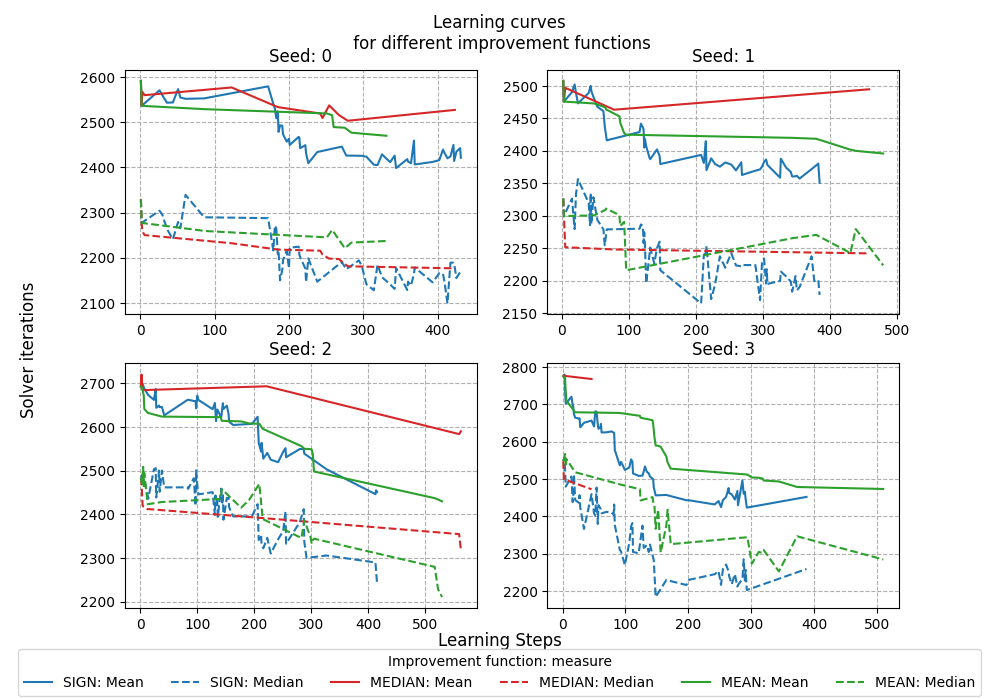
\includegraphics[width=1\textwidth]{plots/improv_func_learn_curve.png}
    \caption{Learning curves for all 12 run configurations. Each plot corresponds to a different seed. The colour of the lines corresponds to a different improvement function: blue for SIGN improvement function; red for MEDIAN improvement function; green for MEAN improvement function. The whole lines is the mean solver iteration count in each learning iteration and the dashed is the median solver iteration count.}
    \label{fig: initial improv learn curve}
\end{figure}

Starting with the MEDIAN improvement function we see from its learning curves in figure \ref{fig: initial improv learn curve}, that it had hard time finding any changes to the preconditioner that would improve the median solver iteration count, with at most 12 accepted preconditioners for seed 0 and down to 3 accepted for seed 3. Table \ref{table: improve func test improvement count} for all acceptance counts. Because of the few number acceptances the evaluation of the preconditioner on the test matrices set, preforms worse in all three measures compared to two other improvement functions for all seeds. Comparing to the unpreconditioned systems the mean and median solver iteration count values are very similar, figure \ref{fig: initial improv test measure}, and only about a fourth of the system have a lower iteration count, figure \ref{fig: initial improv BvN}. With this we can say that the using MEDIAN improvement function in learning does not work. 
\newpage

With MEAN improvement function the problem of few acceptances is not as prevalent, but still happened for seed 0 with 9 instances of improvement occurring. Of the four runs with MEAN improvement function seed 0 is the one that worst in the evaluations of the learned preconditioner mean and median solver iteration count. While int the individual comparison almost a three fourths of the systems have a lower iteration count compared to the unpreconditioned systems for all four seeds. For the other three seeds the learned preconditioners does decrease the solver iteration counts. 

Lastly with SIGN improvement function does not suffer from the problem with few number of improvements, and therefore consistently have a better evaluation of the learned preconditioners. The fluctuations in the learning curves is because of the problem described earlier. From this we can conclude that a preconditioner with this bidiagonal structure can be learned to improve the solver iteration count for an unseen linear systems, with the right improvement function.


\begin{table}[H]
    \center
    \begin{tabular}{|r|r|r|r|}
        \hline
        Seed &SIGN& MEDIAN & MEAN  \\\hline
        0  & 56& 12 & 9 \\
        1  & 60& 5 & 14 \\
        2 & 52 & 7 & 22 \\
        3 & 64& 3 & 25  \\\hline
    \end{tabular}
    \caption{Number of instances a change made to the preconditioner got accepted. A row for each the four seed and columns for each of the three improvement functions.}
    \label{table: improve func test improvement count}
\end{table}



\begin{figure}[H]
    \center
    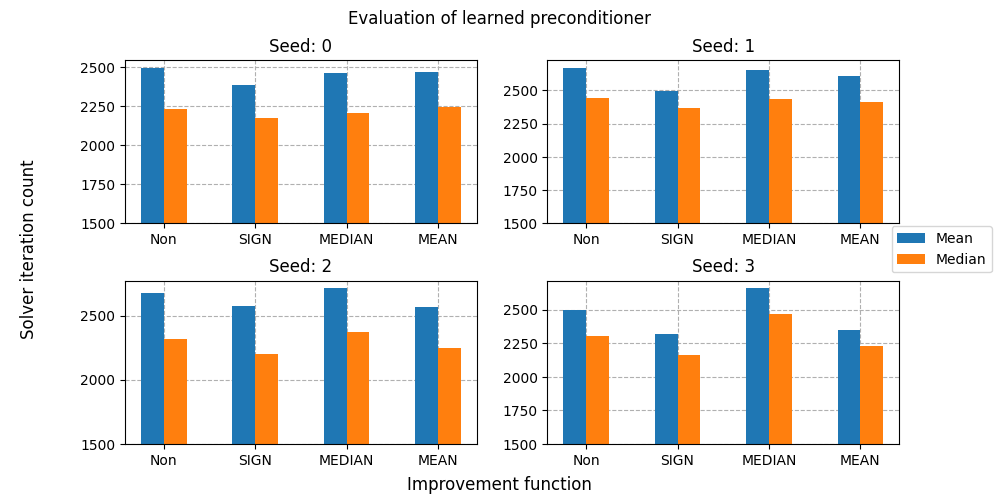
\includegraphics[width=1\textwidth]{plots/improv_func_test_measure.png}
    \caption{Comparison plot of the evaluation of the learned preconditioner where each plot corresponds to a different seed in the learning. The colour of the bars corresponds to the mean solver iteration  count for blue and median solve iteration count for orange. The groups is the different improvement functions used in learning which are in order the unpreconditioned system; SIGN improvement function; MEDIAN as the improvement function; MEAN as the improvement function. Lower is better.}
    \label{fig: initial improv test measure}
\end{figure}



\begin{figure}[H]
    \center
    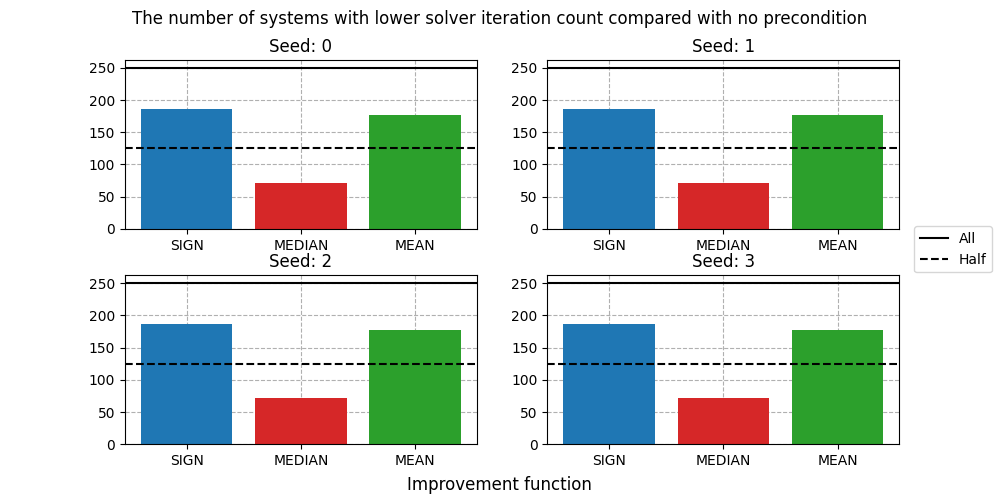
\includegraphics[width=1\textwidth]{plots/improv_func_BvN.png}
    \caption{Bar plot of of many of the system where the preconditioner improved the solver iteration count compared to the unpreconditioned systems. Each plot is for a different seed. The bars corresponds to a different improvement function used in learning indicated by its label. The dashed line is half the data set and full is the whole data set. Higher is better.}
    \label{fig: initial improv BvN}
\end{figure}

